\documentclass[12pt,a4paper]{article}
\usepackage{longtable}
\usepackage[LGR,T1]{fontenc}
\usepackage{lscape}
%\usepackage{pdfsync}
\usepackage{multirow}
\usepackage{amsmath,bm} 
\usepackage{amsfonts}
\usepackage{amsthm} % Extended theorem environments
%\usepackage{amssymb} % Math symbols %%redundant with stix package
%\usepackage{esint} % Intégrales multiples
%\usepackage{esvect} % Vecteurs
\usepackage{mathtools}
\usepackage{pifont} 
 
\usepackage{fancyhdr}
\usepackage{graphicx}

\graphicspath{{../frontend/img/}{../chap_intro_ccl/img/}{../chap_case_study/img/}{../chap_ES_PCE/img/}{../chap_electro_uq/img/}{../chap_methodo/img/}{../chap_myopic/img/}{../chap_RL/img/}{../chap_atom_mol/img/}{../chap_RobPol/img/}{../appendices/img/}} % Figures folder different for each input
%\graphicspath{{img/}} %
\DeclareGraphicsExtensions{.eps,.pdf,.png,.jpg}




\usepackage{lastpage}
\usepackage{afterpage}
\usepackage{lettrine}
\usepackage{color,soul}
\usepackage[dvipsnames]{xcolor}
\usepackage{colortbl}
\usepackage{enumitem}
\usepackage{tikz}
\usepackage{titlesec}
\def\eg{e.g.,\ }
\def\ie{i.e.,\ }


%Palatino font
%\usepackage{pxfonts}
%\usepackage{libertine}
\usepackage[scaled=0.88]{beraserif}
\usepackage[scaled=0.85]{berasans}
\usepackage[scaled=0.84]{beramono}
\usepackage{mathpazo}
%\linespread{1.05}
\usepackage[T1,small,euler-digits]{eulervm}

\usepackage[nomessages]{fp}


\definecolor{bleuUCLclair}{rgb}{.09, 0.569, 1}
\definecolor{bleuUCLfonce}{rgb}{ .13, .52, .86}
\definecolor{redBurn}{rgb}{.91, 0.29, 0.08}

\usepackage{tocloft}
\renewcommand{\cftsecpresnum}{Reviewer \#}
\renewcommand{\cftsecnumwidth}{6em}
\renewcommand{\cftsubsecpresnum}{Comment \#}
\renewcommand{\cftsubsecnumwidth}{6em}

\usepackage[colorlinks=true,urlcolor=black,linkcolor=black,citecolor=black]{hyperref}
\usepackage[square,numbers,sort&compress]{natbib}

\bibliographystyle{biblio/elsarticle-num-names}  %Ordered by appearance in the text, with DOI and URL
%\usepackage[backend=biber, natbib=true, style=numeric-comp, citestyle=numeric-comp, sorting=none, giveninits=true, maxcitenames=1]{biblatex}

\usepackage[]{tocbibind}
\usepackage{hyperref}
\hypersetup{
    colorlinks=true,
%    linkcolor=black,
    bookmarks=true,
    pdfpagemode=FullScreen,
}
\setcounter{tocdepth}{1}

\addtolength{\topmargin}{-1.5cm}
\addtolength{\textheight}{1.5cm}
\addtolength{\textwidth}{2cm}
\addtolength{\footskip}{2cm}
\setlength{\evensidemargin}{-0.5cm}
\setlength{\oddsidemargin}{-0.5cm}
\setlength{\arrayrulewidth}{0.25pt}

\renewcommand{\baselinestretch}{1.1} % Interligne


\newenvironment{maliste}%
{ \begin{list}%
	{\textcolor{bleuUCLfonce}{$\bullet$}\hspace{0.5cm}}%
	{\setlength{\labelwidth}{50pt}%
	 \setlength{\leftmargin}{25pt}%
	 \setlength{\itemsep}{30pt}}}%
{ \end{list} }

%\renewcommand{\headrulewidth}{0.0pt}
%\newcommand{\clearemptydoublepage}{%
%	\newpage{\pagestyle{empty}\cleardoublepage}}




%section like title in longtable
\newcommand{\seclong}[1]{\multicolumn{2}{@{}l}{{\Large\sffamily #1}} 
\vspace{0.5cm}
\\}

%enumerate on two columns
\newcounter{listlong}
\newcommand{\newlistlong}{\setcounter{listlong}{1}}
\newcommand{\iteml}[1]{%
\hspace{4.5cm}\textcolor{redBurn}{\arabic{listlong}}\stepcounter{listlong}%
&%
#1%
 
\\%
}

%left in column
\newcommand{\lcol}[1]{%
\begin{minipage}[t]{.35\textwidth}%

#1%

\end{minipage}%
}

\title{\vspace{-1cm}
\begin{flushleft} {\sffamily Xavier Rixhon's PhD thesis - Answers to jury members}\end{flushleft}}
\date{\vspace{-1.7cm}\begin{flushleft}\sffamily Exploration of uncertainty-aware energy transition pathways - Reinforcement learning and principal component analysis-based methods\end{flushleft}}
%
%Xavier Rixhon, Gauthier Limpens, Diederik Coppitters, Hervé Jeanmart and Francesco Contino\end{flushleft}}


\pagestyle{fancy} 
\fancyhf{}
\fancyfoot[R]{\sffamily\thepage\ / \pageref{LastPage}}
  \fancyfoot[L]{ }

\fancypagestyle{plain}{%
  \fancyhf{}%
  \fancyfoot[R]{\sffamily\thepage\ / \pageref{LastPage}}
  \fancyfoot[L]{ }
}

\renewcommand{\headrulewidth}{0.0pt}


\newcommand{\hlc}[2][yellow]{ {\sethlcolor{#1} \hl{#2}} }

\titleformat{\section}
  {\bfseries\scshape}{}{1em}{}

\titleformat{\subsection}
  {\normalfont\scshape}{}{1em}{}

\usepackage[framemethod=default]{mdframed}
%\mdfsetup{skipabove=\topskip,skipbelow=\topskip}

\global\mdfdefinestyle{comment}{%
     linecolor=red,linewidth=0.1cm,%
     leftmargin=-0.5cm,rightmargin=-0.5cm, innerleftmargin=0.4cm,innerrightmargin=0.4cm,
     topline=false,bottomline=false
}

\global\mdfdefinestyle{manuscript}{%
     linecolor=gray!20,linewidth=0.05cm,backgroundcolor=gray!20,%
     leftmargin=-0.5cm,rightmargin=-0.5cm, innerleftmargin=0.4cm,innerrightmargin=0.4cm
}
  
  \renewcommand{\subsectionautorefname}{Comment}
\begin{document}
\maketitle

I would like to thank the jury members for the comments, which significantly helped improving the manuscript and substantiating the novelty of my work. Based on the notes taken during the private defense, I hereby transcribed, as accurately as possible, the jury's comments. 

I believe I have addressed all the issues raised in the following answers. Some of them required adaptations of the text. These adaptations are either directly in the thesis manuscript or left for further developments in subsequent papers. For each comment, I have first highlighted the issue, then provided an answer, and finally described how the manuscript was adjusted, if needed.\\

When a comment explicitly comes from specific members of the jury, they are listed at the beginning of the comment with the following color code: {\color{orange} \textbf{Stefano} Moret}, {\color{teal} \textbf{Stefan} Pfenninger}, {\color{purple} \textbf{Sylvain} Quoilin} and {\color{violet} \textbf{Christophe} De Vleeschouwer}. Here is how an answer to a comment is structured:

\begin{mdframed}[style=comment] % Comment from the reviewer
Text of the comment. When a page number is mentioned at the beginning of the comment, it refers to the page number of the manuscript submitted before the private defense, not its final version.
\end{mdframed}

\noindent The answer provided to the comment and, based on this, where the potential modification brought to the manuscript is located in the thesis manuscript using {\color{blue} blue font}.

\begin{mdframed}[style=manuscript] % Modification brought to the manuscript
New version of the text in the manuscript.
\end{mdframed}

% {\color{orange} \textbf{Stefano}}
% {\color{purple} \textbf{Sylvain}}
% {\color{teal} \textbf{Stefan}}
% {\color{violet} \textbf{Christophe}}

\clearpage

\section{General comments/questions}
\label{General}

\begin{mdframed}[style=comment] % Comment from the reviewer
{\color{orange} \textbf{Stefano}} - Overall, many methods: PCE + RL + NN + PCA. At each stage, some assumption is made. Why not a simpler approach or a simpler model? Do you need all these steps? Explain the role of the different methods and why PCE instead of monthly version for uncertainty? 
\end{mdframed}

\noindent

\begin{mdframed}[style=manuscript] % Comment from the reviewer

\end{mdframed}

\begin{mdframed}[style=comment] % Comment from the reviewer
{\color{violet} \textbf{Christophe}} - The variables and the uncertainties should be presented in a compact and mathematical way.
\end{mdframed}

\noindent

\begin{mdframed}[style=manuscript] % Comment from the reviewer

\end{mdframed}


\subsection{Assumptions - Fine tuning}
\label{fine_tuning}

\begin{mdframed}[style=comment] % Comment from the reviewer
{\color{orange} \textbf{Stefano}}, {\color{purple} \textbf{Sylvain}} \& {\color{teal} \textbf{Stefan}} - Many assumptions, e.g., alpha = 85\% (p. 40) or reward = -300 (Chapter 4). How sensitive are the results to these assumptions? It looks like all these parameters have been tuned to obtain the desired results. How robust are they? Can the methodology be generalized to other models? Can we keep the same values for other applications? You need a model that runs pretty fast, right?
\end{mdframed}

\noindent Perhaps there is a need to better prove or show that it is not a magic number.  How to generalise it and hook it to something physical (even if it is done a posteriori). Guidelines to apply it to some other models

\begin{mdframed}[style=manuscript] % Comment from the reviewer

\end{mdframed}

\begin{mdframed}[style=comment] % Comment from the reviewer
{\color{purple} \textbf{Sylvain}} - Make sure to discuss the hypotheses because one might not agree with all of them. So, it could provide more context but also some limitations and indications of the alternatives (and the spectrum of what is possible).
\end{mdframed}

\noindent

\begin{mdframed}[style=manuscript] % Comment from the reviewer

\end{mdframed}



\subsection{Graphs and results}
\label{general_graphs_results}

\begin{mdframed}[style=comment] % Comment from the reviewer
{\color{orange} \textbf{Stefano}}, {\color{teal} \textbf{Stefan}} \& {\color{purple} \textbf{Sylvain}} - Graphs like the ones presented during the private defense (slides 19, 22 and 24) should be better explained. Many axes labels are missing, and the captions are often insufficient to read the figures. In general, improve the presentation of the results, especially for the RL chapter.
\end{mdframed}

\noindent

\begin{mdframed}[style=manuscript] % Comment from the reviewer

\end{mdframed}

\begin{mdframed}[style=comment] % Comment from the reviewer
{\color{orange} \textbf{Stefano}} - Work on the graph of slide 19 (there is a misunderstanding on the fact that the grey curve is labelled as failure but they are failures in the future)
\end{mdframed}

\noindent Make the link with the success rate (during the training).  To be discussed to keep most of the attemps even though they are discarded

\begin{mdframed}[style=manuscript] % Comment from the reviewer

\end{mdframed}

\begin{mdframed}[style=comment] % Comment from the reviewer
{\color{teal} \textbf{Stefan}} - Some big topics are missing like storage. Why is storage not more discussed? 
\end{mdframed}

\noindent Storage is a by-product of the results and they’re barely affected by the different studies. It’s mostly gas storage (on average 18TWh) and, to a smaller extent, seasonal thermal storage.

\begin{mdframed}[style=manuscript] % Comment from the reviewer

\end{mdframed}

\begin{mdframed}[style=comment] % Comment from the reviewer
{\color{teal} \textbf{Stefan}} - What is the potential of what we can learn from the results of the innovative methods? We could go further in the analysis as we know we have to phase out coal, install renewables.
\end{mdframed}

\noindent The outcome is a bit too obvious (e.g. getting rid of the coal) $\rightarrow$ go a bit in the details. Explain why the method is taking better decisions but explain why. $\rightarrow$ go beyond what we know

\begin{mdframed}[style=manuscript] % Comment from the reviewer

\end{mdframed}

\subsection{Structure}
\label{structure}

\begin{mdframed}[style=comment] % Comment from the reviewer
{\color{orange} \textbf{Stefano}} \& {\color{teal} \textbf{Stefan}} - The thesis structure makes it quite difficult to follow. Having all the methodology summarised in Chapter 1, makes it difficult to link it to the different chapters. As changing the structure may be now a major work, I would invite you to think how to better connect the different parts. 
\end{mdframed}

\noindent Initially, I wanted to group methodology and results per kind of analysis, \ie UQ on Pathway (Chapter 3), RL (Chapter 4) and PCA (Chapter 5) but that would have made the RL, and even more PCA, methodology parts come too far in the manuscript. For this reason, I made the choice to group all the methodological approaches together in Chapter 1 and the results in their respective chapter. 

\begin{mdframed}[style=manuscript] % Comment from the reviewer

\end{mdframed}

\subsection{References}
\label{references}

\begin{mdframed}[style=comment] % Comment from the reviewer
{\color{orange} \textbf{Stefano}} \& {\color{purple} \textbf{Sylvain}} - I found it unusual to see many references to own work (Rixhon et al.) throughout the thesis. Unless the articles are unrelated to the thesis, these references should be removed and the associated content should be included in the manuscript. As an example, at p. 25, results are mentioned which are not reported in the thesis. The reader currently must refer to [48] to see these results, which should instead be included in the thesis. 
\end{mdframed}

\noindent

\begin{mdframed}[style=manuscript] % Comment from the reviewer

\end{mdframed}

\begin{mdframed}[style=comment] % Comment from the reviewer
{\color{violet} \textbf{Christophe}} - State of the art mainly European. Why not reference to other regions of the world.
\end{mdframed}

\noindent
It is an interesting topic for further investigations, especially how they address the subject in other parts of the world like Australia/Asia. This could be linked with the political perception of energy system optimisation models and the subsequent analyses. However, no modification has been brought to the manuscript regarding this topic.

\subsection{Writing style}
\label{writing_style}

\begin{mdframed}[style=comment] % Comment from the reviewer
{\color{orange} \textbf{Stefano}} -While a more ``friendly'' writing style can be pleasant, there are many colloquial expressions that not do not fit well in the thesis, \eg ``carrot and stick'', ``apples with apples'', etc. I recommend reducing them to the bare minimum, or completely getting rid of them. 
\end{mdframed}

\noindent

\begin{mdframed}[style=manuscript] % Comment from the reviewer

\end{mdframed}

\begin{mdframed}[style=comment] % Comment from the reviewer
There are various typos in the thesis, e.g. ``storagR'' (page 3), ``therefore, therefore'' (p. 11), ``The'' (p.14), ``Moleclues'' (p. 61), etc.. Also, the use English language can be improved, e.g. ``calls FOR a variety'' (p. 9), ``cumulative emissions ARE'' (p. 14), ``than to'' (p. 34), etc. The document will benefit from a spelling/grammar check.
\end{mdframed}

\noindent

\begin{mdframed}[style=manuscript] % Comment from the reviewer

\end{mdframed}

\subsection{Documentation}
\label{documentation}

\begin{mdframed}[style=comment] % Comment from the reviewer
{\color{purple} \textbf{Sylvain}} - Where is the repository for the code? Don't forget the documentation?
\end{mdframed}

\noindent As discussed during the private defense, this is a task that is already planned for the year to come, after the public defense. A better reference towards these repository and documentation will be given in the subsequent paper on RL. Consequently, there has not been further work done in this regard in the manuscript by the public defense.

\section{Introduction}
\label{Introduction}

\begin{mdframed}[style=comment] % Comment from the reviewer
{\color{orange} \textbf{Stefano}} \& {\color{teal} \textbf{Stefan}} - At page 1, it is mentioned that you focus on the technical levers of the transition, ``renewables'' and ``efficiency''. From this I understand that you are not focusing on ``sufficiency''. This seems to contradict a statement at p. 2, where it is mentioned that one objective of the thesis is to ``support interdisciplinary projects in the assessment of sufficiency policy''. I suggest clarifying this potential misunderstanding.  
\end{mdframed}

\noindent I totally agree with this remark, especially because I do not want to overlook the necessary third pillar of the transition which is ``sufficiency'', even though my thesis does not address directly this aspect. Consequently, I have adapted {\color{blue} page 2 of the introduction}:

\begin{mdframed}[style=manuscript] % Modification brought to the manuscript
Among all the lenses through which it is necessary to assess sufficiency policies, one of the objectives of this work is to support these interdisciplinary projects by providing informed techno-economic guidelines.
\end{mdframed}

\noindent This technical contribution to the interdisciplinary debate of sufficiency is reminded in {\color{blue} the last sentence of the conclusion}.

\begin{mdframed}[style=manuscript] % Modification brought to the manuscript
In this sense, this work provided insight about possible transition pathways for Belgium to bring the technical dimension into the intrinsically political and interdisciplinary discussions and decisions that must be made in the coming years.
\end{mdframed}

\section{Chapter 1 - Methodology}
\label{methodo}

\subsection{EnergyScope Pathway}
\label{ESPathway}
\begin{mdframed}[style=comment] % Comment from the reviewer
{\color{orange} \textbf{Stefano}} - p.11 : The stated computational time seems low for a pathway model with hourly resolution. Were there approximations (e.g., disabling crossover) added and what was their impact?\end{mdframed}

\noindent 

\begin{mdframed}[style=manuscript] % Modification brought to the manuscript

\end{mdframed}

\begin{mdframed}[style=comment] % Comment from the reviewer
{\color{orange} \textbf{Stefano}} - Can you explain the logic of the annualization factor in the pathway model and the choice of N=5 for the uncertainty ranges?
\end{mdframed}

\noindent 

\begin{mdframed}[style=manuscript] % Modification brought to the manuscript

\end{mdframed}

\subsubsection{End-of-time-horizon and salvage value}


\begin{mdframed}[style=comment] % Comment from the reviewer
{\color{orange} \textbf{Stefano}} - Often, multi-stage models are affected by the end-of-time-horizon effects. Did you observe those and how did you deal with them? See, e.g. Figure 3.3 p. 66.
\end{mdframed}

% \noindent Better highlight the importance, discuss the finetuning, discuss  alternatives (e.g. adding time windows at the end that are thrown afterwards).

\begin{mdframed}[style=manuscript] % Modification brought to the manuscript

\end{mdframed}

\begin{mdframed}[style=comment] % Comment from the reviewer
{\color{teal} \textbf{Stefan}} - The salvage value plays a large role in the decision of the model. Give more details to give more confidence in the choice.
\end{mdframed}

\noindent See what's been written in appendix paper Pathway

\begin{mdframed}[style=manuscript] % Modification brought to the manuscript

\end{mdframed}

\subsubsection{Myopic pathway}

\begin{mdframed}[style=comment] % Comment from the reviewer
{\color{orange} \textbf{Stefano}} - p.17-19: is the myopic version modeled as a single LP or as a sequence of LPs? This should be better clarified. The diagram at p. 19 focuses on the code, it would be better replaced by a code showcasing the logic of the approach.
\end{mdframed}

\noindent 

\begin{mdframed}[style=manuscript] % Modification brought to the manuscript

\end{mdframed}

\begin{mdframed}[style=comment] % Comment from the reviewer
{\color{teal} \textbf{Stefan}} - With the myopic approach, are you predicting what will come or drawing a path that is the best? Is that a desirable feature to mimic the way we proceed now. why artificially limit the model as we know we have to go to zero in 2050.
\end{mdframed}

\noindent Link to salvage value

\begin{mdframed}[style=manuscript] % Modification brought to the manuscript

\end{mdframed}

\begin{mdframed}[style=comment] % Comment from the reviewer
{\color{teal} \textbf{Stefan}} - p.18 : Surprising that myopic leads to a sooner investment to the transition ? Is it an effect of the salvage value? was there a sensitivity analysis on this salvage value? Perhaps include more details on this.
\end{mdframed}

\noindent 

\begin{mdframed}[style=manuscript] % Modification brought to the manuscript

\end{mdframed}

\subsubsection{Discount rate and annualization}

\begin{mdframed}[style=comment] % Comment from the reviewer
{\color{purple} \textbf{Sylvain}} - Wouldn't it be more appropriate to talk about ``discount rate'' rather than ``interest rate''?
\end{mdframed}

\noindent Indeed, as we want to capture the time preference associated with obtaining finance for the project, effectively quantifying the trade-off between present and future financial value, it is more appropriate to refer to ``discount rate'' when considering the parameter $i_{\text{rate}}$. We have changed every occurrence of ``interest rate'' into ``discount rate'' {\color{blue}in the entire manuscript}.

\begin{mdframed}[style=comment] % Comment from the reviewer
{\color{purple} \textbf{Sylvain}} - Value of the discount rate is generally above 6\% in other works. You should have a better justification of selecting 1.5\%.
\end{mdframed}

\noindent  {\color{blue} }.

\begin{mdframed}[style=manuscript] % Modification brought to the manuscript 

\end{mdframed}

\begin{mdframed}[style=comment] % Comment from the reviewer
{\color{purple} \textbf{Sylvain}} - p.13 - Why no annualizing over the lifetime of the unit? Would that lead to different results? 
\end{mdframed}

\noindent {\color{blue} }.

\begin{mdframed}[style=manuscript] % Modification brought to the manuscript 

\end{mdframed}

\subsubsection{Power grid and transport infrastructure}

\begin{mdframed}[style=comment] % Comment from the reviewer
{\color{purple} \textbf{Sylvain}} - How do you model the power grid interconnections with the neighbouring countries as well as the transport network of the different energy carriers within the country?
\end{mdframed}

\noindent Copper-plate assumption $\rightarrow$ no representation of the transport sector of either electricity or gaseous and liquid energy carriers. However, one technology called ``GRID'' accounts for the additional investments in the power grid needed when deploying more VRES like PV panels and wind turbines but there is not an actual spatial representation of this grid. {\color{blue} }.

\begin{mdframed}[style=manuscript] % Modification brought to the manuscript 

\end{mdframed}

\subsection{Uncertainty quantification}
\label{methodo_UQ}

\begin{mdframed}[style=comment] % Comment from the reviewer
{\color{orange} \textbf{Stefano}} - p. 20: “inspired by Guevara et al.” $\rightarrow$ how was their approach used in your work?
\end{mdframed}

\noindent 

\begin{mdframed}[style=manuscript] % Modification brought to the manuscript

\end{mdframed}

\begin{mdframed}[style=comment] % Comment from the reviewer
{\color{orange} \textbf{Stefano}} - p. 21: footnote. The statement is qualitative, it should be quantitative. What is the minimum number of runs needed to validate your experiments? Did you look into that? How was the surrogate model validated?
\end{mdframed}

\noindent 

\begin{mdframed}[style=manuscript] % Modification brought to the manuscript

\end{mdframed}

\begin{mdframed}[style=comment] % Comment from the reviewer
{\color{orange} \textbf{Stefano}} - p. 23: is PCE an appropriate method for LP / MILP models. There is a good fit (1\% LLO error) for the total cost, which is often quite linear, but how about technology choice / sizing?
\end{mdframed}

\noindent Expand on this in the chapter while acknowledging the limitations and saying it is not the main topic of the thesis. 

\begin{mdframed}[style=manuscript] % Modification brought to the manuscript

\end{mdframed}

\begin{mdframed}[style=comment] % Comment from the reviewer
{\color{orange} \textbf{Stefano}} - p. 24: Sobol indices. Can you explain the choice wrt other methods? Difference between factor prioritization and factor fixing?
\end{mdframed}

\noindent 

\begin{mdframed}[style=manuscript] % Modification brought to the manuscript

\end{mdframed}

\begin{mdframed}[style=comment] % Comment from the reviewer
{\color{orange} \textbf{Stefano}} - Why is PCE needed is EnergyScope is already very fast?
\end{mdframed}

\noindent 

\begin{mdframed}[style=manuscript] % Modification brought to the manuscript

\end{mdframed}

\begin{mdframed}[style=comment] % Comment from the reviewer
{\color{purple} \textbf{Sylvain}} - p.21 - How are the groups of uncertainties defined? Is there a table?
\end{mdframed}

\noindent {\color{blue} }.

\begin{mdframed}[style=manuscript] % Modification brought to the manuscript 

\end{mdframed}

\begin{mdframed}[style=comment] % Comment from the reviewer
{\color{purple} \textbf{Sylvain}} - Table 1.2 - what are the other parameters?
\end{mdframed}

\noindent {\color{blue} }.

\begin{mdframed}[style=manuscript] % Modification brought to the manuscript 

\end{mdframed}

\subsection{Reinforcement Learning}
\label{methodo_RL}

\begin{mdframed}[style=comment] % Comment from the reviewer
{\color{orange} \textbf{Stefano}} - p. 31: Can you explain the need of using NN here? Couldn’t you just run the energyscope model?
\end{mdframed}

\noindent 

\begin{mdframed}[style=manuscript] % Modification brought to the manuscript

\end{mdframed}

\begin{mdframed}[style=comment] % Comment from the reviewer
{\color{purple} \textbf{Sylvain}} - p. 27 When presenting the advantages of RL, you mention model-free approach. Ok, but you have a representation of the real world available to train the model!
\end{mdframed}

\noindent {\color{blue} }.

\begin{mdframed}[style=manuscript] % Modification brought to the manuscript 

\end{mdframed}

\begin{mdframed}[style=comment] % Comment from the reviewer
{\color{teal} \textbf{Stefan}} - Justification of the actions selected? why no other actions like the cost of some technologies? 
\end{mdframed}

\noindent These actions have a direct translation in constraints and we can therefore assess their effectiveness through the fact they are binding or not. Give examples of actions tried during the work (incentivize renewables) or other from Assemblée citoyenne in France and explain why they’re not as good as those chosen in the thesis. Explain history of what we tried/consider? 
 {\color{blue} }.

\begin{mdframed}[style=manuscript] % Modification brought to the manuscript 

\end{mdframed}

\subsection{Principal Component Analysis}
\label{methodo_PCA}

\begin{mdframed}[style=comment] % Comment from the reviewer
{\color{orange} \textbf{Stefano}} - p. 32: Why is PCA needed? Wouldn’t it be easier to just aggregate similar outputs of interest?
\end{mdframed}

\noindent 

\begin{mdframed}[style=manuscript] % Modification brought to the manuscript

\end{mdframed}

\begin{mdframed}[style=comment] % Comment from the reviewer
{\color{orange} \textbf{Stefano}} - p. 42: Figure 1.17. What is your definition of robustness? Having a tight distribution but all shifted towards very suboptimal costs seems to fit your definition. Please clarify.
\end{mdframed}

\noindent 

\begin{mdframed}[style=manuscript] % Modification brought to the manuscript

\end{mdframed}

\begin{mdframed}[style=comment] % Comment from the reviewer
{\color{purple} \textbf{Sylvain}} - p. 39 Why are their outliers in the first case? Isn't a bit arbitrary to set them to a min/max value?
\end{mdframed}

\noindent I should insist on those elements in the text {\color{blue} }.

\begin{mdframed}[style=manuscript] % Modification brought to the manuscript 

\end{mdframed}

\section{Chapter 2 - Case study}
\label{methodo}

\begin{mdframed}[style=comment] % Comment from the reviewer
{\color{orange} \textbf{Stefano}} - I am a bit underwhelmed by the many nitty-gritty data in this Chapter. While it is surely important to document everything, couldn’t at least part of this be moved to the Appendix?\end{mdframed}

\noindent 

\begin{mdframed}[style=manuscript] % Modification brought to the manuscript

\end{mdframed}

\begin{mdframed}[style=comment] % Comment from the reviewer
{\color{orange} \textbf{Stefano}} - Figure 2.5: What is the purpose of the violet line between ``biomass gasification'' and ``methanolation''?
\end{mdframed}

\noindent These were actually two different arrows, one pointing from ``biomass gasification for CH3OH'' to ``Methanol'' and the other from ``Methanolation'' to ``Methanol''. To avoid this confusion, the figure has been updated and the origin of these arrows are now on different vertical levels {\color{blue} see Section 2.3}.

\begin{figure}[htbp!]
\centering
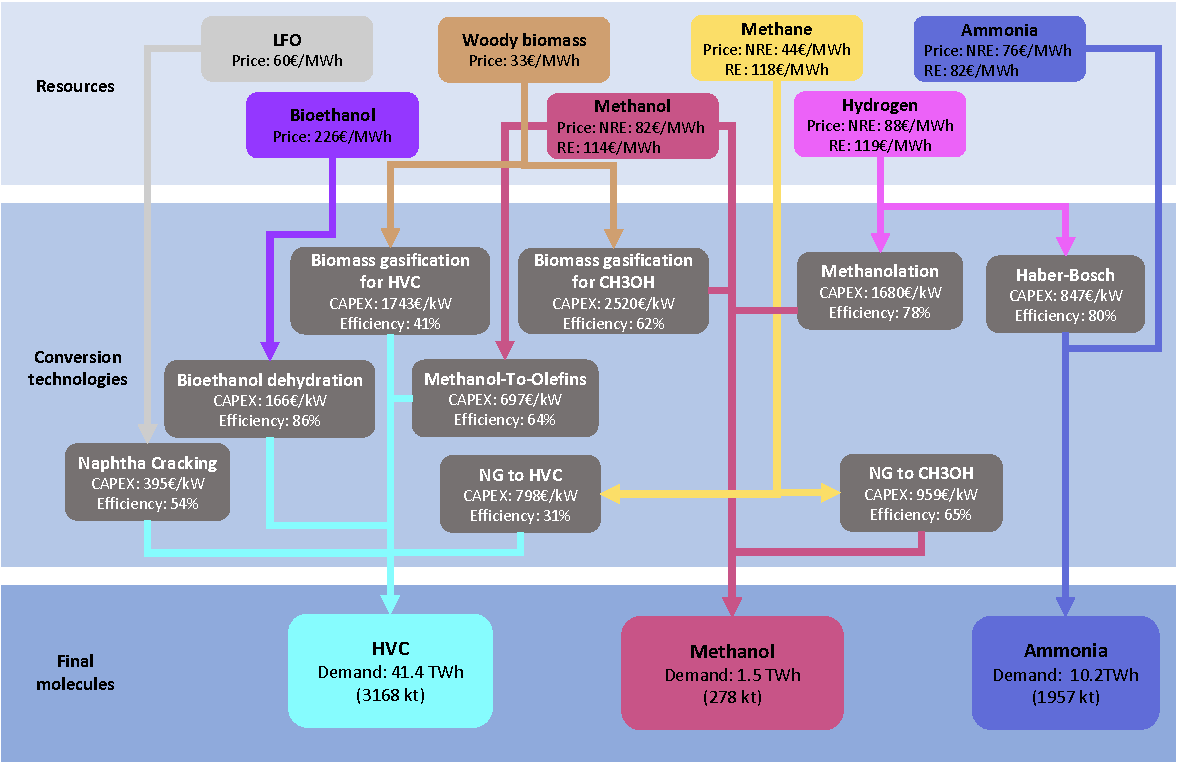
\includegraphics[width=\textwidth]{NED_tech.pdf}
\label{fig:NED_tech}
\end{figure}

\begin{mdframed}[style=comment] % Comment from the reviewer
{\color{purple} \textbf{Sylvain}} - p. 45 How is the range accounted for the characterisation of private mobility technologies?
\end{mdframed}

\noindent Indeed, the increase of the range is a consequence of the increased efficiency and battery capacity. Consequently, I have removed the mention to the range {\color{blue}at the end of the last paragraph in the contributions of Chapter 2}.

\begin{mdframed}[style=manuscript] % Modification brought to the manuscript 
Regarding BEV, while the CAPEX has been kept unchanged, the efficiency and the battery capacity have been increased. 
\end{mdframed}

\begin{mdframed}[style=comment] % Comment from the reviewer
{\color{purple} \textbf{Sylvain}} - p. 51 Offshore wind max capacity is too low and PV is lower than Bregilab
\end{mdframed}

\noindent {\color{blue} }.

\begin{mdframed}[style=manuscript] % Modification brought to the manuscript 

\end{mdframed}

\begin{mdframed}[style=comment] % Comment from the reviewer
{\color{purple} \textbf{Sylvain}} - p. 51 Offshore wind max capacity is too low and PV is lower than Bregilab
\end{mdframed}

\noindent {\color{blue} }.

\begin{mdframed}[style=manuscript] % Modification brought to the manuscript 

\end{mdframed}

\begin{mdframed}[style=comment] % Comment from the reviewer
{\color{purple} \textbf{Sylvain}} - p. 51 Why investigating SMR?
\end{mdframed}

\noindent {\color{blue} }.

\begin{mdframed}[style=manuscript] % Modification brought to the manuscript 

\end{mdframed}

\begin{mdframed}[style=comment] % Comment from the reviewer
{\color{purple} \textbf{Sylvain}} - p. 51 Last paragraph of p. 51 is not clear. Are we talking about the purchase cost or the CO2 content?
\end{mdframed}

\noindent {\color{blue} }.

\begin{mdframed}[style=manuscript] % Modification brought to the manuscript 

\end{mdframed}

\begin{mdframed}[style=comment] % Comment from the reviewer
{\color{purple} \textbf{Sylvain}} - p. 53 4850€/kW is at the lower end of the EnergyVille scenario for SMR (4500€/kW).
\end{mdframed}

\noindent {\color{blue} }.

\begin{mdframed}[style=manuscript] % Modification brought to the manuscript 

\end{mdframed}

\begin{mdframed}[style=comment] % Comment from the reviewer
{\color{purple} \textbf{Sylvain}} - p. 53 What about fuel cost? This is a very optimistic price forecast! 
\end{mdframed}

\noindent {\color{blue} }.

\begin{mdframed}[style=manuscript] % Modification brought to the manuscript 

\end{mdframed}

\begin{mdframed}[style=comment] % Comment from the reviewer
{\color{purple} \textbf{Sylvain}} - p. 53 Do the parameters of the uncertainty analysis arrive later on?
\end{mdframed}

\noindent {\color{blue} }.

\begin{mdframed}[style=manuscript] % Modification brought to the manuscript 

\end{mdframed}

\begin{mdframed}[style=comment] % Comment from the reviewer
{\color{purple} \textbf{Sylvain}} - p. 54 Is there a differentiation between ground mounted and rooftop PV?
\end{mdframed}

\noindent {\color{blue} }.

\begin{mdframed}[style=manuscript] % Modification brought to the manuscript 

\end{mdframed}

\begin{mdframed}[style=comment] % Comment from the reviewer
{\color{purple} \textbf{Sylvain}} - p. 54 Current tenders for 3rd generation are higher than 100€/MWh. There are papers showing that SMRs are not really expected to be cheaper than 3rd generation. How realistic is 41 €/MWh?
\end{mdframed}

\noindent {\color{blue} }.

\begin{mdframed}[style=manuscript] % Modification brought to the manuscript 

\end{mdframed}

\begin{mdframed}[style=comment] % Comment from the reviewer
{\color{purple} \textbf{Sylvain}} - p. 54 LCOE of SMRs would be much lower if: - the capital cost was more realistic and, - the Capacity factor was lowered to account for their flexible use.
\end{mdframed}

\noindent {\color{blue} }.

\begin{mdframed}[style=manuscript] % Modification brought to the manuscript 

\end{mdframed}

\begin{mdframed}[style=comment] % Comment from the reviewer
{\color{purple} \textbf{Sylvain}} - p. 55 - Figure 2.5 - Coupled with heat for endogenous and exogenous reactions?
\end{mdframed}

\noindent {\color{blue} }.

\begin{mdframed}[style=manuscript] % Modification brought to the manuscript 

\end{mdframed}

\begin{mdframed}[style=comment] % Comment from the reviewer
{\color{purple} \textbf{Sylvain}} - p. 56 Are modal shares exogenously set?
\end{mdframed}

\noindent {\color{blue} }.

\begin{mdframed}[style=manuscript] % Modification brought to the manuscript 

\end{mdframed}

\begin{mdframed}[style=comment] % Comment from the reviewer
{\color{purple} \textbf{Sylvain}} - p. 57 Why a uniform distribution? A gaussian woul clearly be more appropriate. Maybe some uncertainties are underestimated (because clipped by uniform distribution)
\end{mdframed}

\noindent {\color{blue} }.

\begin{mdframed}[style=manuscript] % Modification brought to the manuscript 

\end{mdframed}

\section{Chapter 3 - Atom-vs-molecules}
\label{Chap_atom_vs_molecules}
\begin{mdframed}[style=comment] % Comment from the reviewer
{\color{orange} \textbf{Stefano}} - Would it be fair to say that the scope of this Chapter is adding one technology (SMR) to the model? Is this a significant contribution?
\end{mdframed}

\noindent 

\begin{mdframed}[style=manuscript] % Modification brought to the manuscript

\end{mdframed}

\begin{mdframed}[style=comment] % Comment from the reviewer
{\color{orange} \textbf{Stefano}} - What is the learning of this chapter? I was underwhelmed by the long list of results. What is the take-away?
\end{mdframed}

\noindent 

\begin{mdframed}[style=manuscript] % Modification brought to the manuscript

\end{mdframed}

\begin{mdframed}[style=comment] % Comment from the reviewer
{\color{orange} \textbf{Stefano}} - p. 70: ``in other words, the variation of the parameter f$\_$max,SMR…''. I am not sure that this sentence is equivalent to the previous one. Please clarify.
\end{mdframed}

\noindent 

\begin{mdframed}[style=manuscript] % Modification brought to the manuscript

\end{mdframed}

\begin{mdframed}[style=comment] % Comment from the reviewer
{\color{orange} \textbf{Stefano}} - p. 71, Table 3.1: isn’t the low impact simply due to the low assumed potential? Is this finding meaningful?
\end{mdframed}

\noindent 

\begin{mdframed}[style=manuscript] % Modification brought to the manuscript

\end{mdframed}

\begin{mdframed}[style=comment] % Comment from the reviewer
{\color{orange} \textbf{Stefano}} - p. 74, Figure 3.8: this graphs looks potentially interesting but it is not sufficiently well explained.
\end{mdframed}

\noindent 

\begin{mdframed}[style=manuscript] % Modification brought to the manuscript

\end{mdframed}

\begin{mdframed}[style=comment] % Comment from the reviewer
{\color{purple} \textbf{Sylvain}} - p. 63 What does efficiency change in the installed capacity?
\end{mdframed}

\noindent Indeed, the efficiency only has an impact on the amount of primary uranium needed to produce the electricity. Consequently, I have removed this part of the sentence {\color{blue}in the first paragraph of Section 3.1.1}. 

\begin{mdframed}[style=manuscript] % Modification brought to the manuscript 
Overall, given the restriction on yearly availability and the slightly higher electrification [...]
\end{mdframed}

\begin{mdframed}[style=comment] % Comment from the reviewer
{\color{purple} \textbf{Sylvain}} - p. 64 - 15 GW of PV in 2025. Realistic?
\end{mdframed}

\noindent {\color{blue} }. 

\begin{mdframed}[style=manuscript] % Modification brought to the manuscript 

\end{mdframed}

\begin{mdframed}[style=comment] % Comment from the reviewer
{\color{purple} \textbf{Sylvain}} - p. 65 - Decides to use ammonia instead of SNG => is the transport infrastructure accounted for?
\end{mdframed}

\noindent {\color{blue} }. 

\begin{mdframed}[style=manuscript] % Modification brought to the manuscript 

\end{mdframed}

\begin{mdframed}[style=comment] % Comment from the reviewer
{\color{purple} \textbf{Sylvain}} - p. 67 - It really depends on what is considered primary energy in the case of nuclear
\end{mdframed}

\noindent {\color{blue} }. 

\begin{mdframed}[style=manuscript] % Modification brought to the manuscript 

\end{mdframed}

\begin{mdframed}[style=comment] % Comment from the reviewer
{\color{purple} \textbf{Sylvain}} - p. 69 - No curtailment at all? It would be nice to have the exact number.
\end{mdframed}

\noindent {\color{blue} }. 

\begin{mdframed}[style=manuscript] % Modification brought to the manuscript 

\end{mdframed}

\begin{mdframed}[style=comment] % Comment from the reviewer
{\color{purple} \textbf{Sylvain}} - p. 69 - Very strange. Should be the same as for industrial boilers. No smart charging?
\end{mdframed}

\noindent {\color{blue} }. 

\begin{mdframed}[style=manuscript] % Modification brought to the manuscript 

\end{mdframed}

\begin{mdframed}[style=comment] % Comment from the reviewer
{\color{purple} \textbf{Sylvain}} - p. 70 - But that's because the CAPEX is way too low. With more realistic values, the Sobol would be much higher.
\end{mdframed}

\noindent {\color{blue} }. 

\begin{mdframed}[style=manuscript] % Modification brought to the manuscript 

\end{mdframed}

\begin{mdframed}[style=comment] % Comment from the reviewer
{\color{purple} \textbf{Sylvain}} - p.71 - Differentiated discount rates could be useful.
\end{mdframed}

\noindent As written in Chapter 3: ``In practice, the discount rate would vary depending on the technology investment risk''. Depending on the technology readiness level, private investors would be more or less risk-averse. However, EnergyScope only considers a vision of a central-planner where a single agent makes the investment decisions without differentiating the sources of the capitals, \ie private and public. Assuming a differentiated discount rate would require to make assumptions about the private-public distribution of the capitals. These further explanations for keeping a single value of discount rate have been added {\color{blue} after Eq. (1.3) when discussing the annualised phase factor}.

\begin{mdframed}[style=manuscript] % Modification brought to the manuscript 
The discount rate accounted for in the annualisation factor is considered as identical for all the technologies of the system. In practice, the discount rate would vary depending on the technology investment risk. Depending on the technology readiness level, private investors would be more or less risk-averse. However, EnergyScope only considers the vision of a central-planner where a single agent makes the investment decisions without differentiating the sources of the capitals, \ie private and public. Assuming a differentiated discount rate would require to make assumptions about the private-public distribution of the capitals. For this reason, we have decided to keep an identical value of discount rate for all the technologies.
\end{mdframed}

\begin{mdframed}[style=comment] % Comment from the reviewer
{\color{purple} \textbf{Sylvain}} - p. 72 - Battery trucks are gaining momentum. Is the hydrogen route really the way to go?
\end{mdframed}

\noindent {\color{blue} }. 

\begin{mdframed}[style=manuscript] % Modification brought to the manuscript 

\end{mdframed}

\begin{mdframed}[style=comment] % Comment from the reviewer
{\color{purple} \textbf{Sylvain}} - p. 73 - How is the transport infrastructure accounted for?
\end{mdframed}

\noindent {\color{blue} }. 

\begin{mdframed}[style=manuscript] % Modification brought to the manuscript 

\end{mdframed}

\begin{mdframed}[style=comment] % Comment from the reviewer
{\color{purple} \textbf{Sylvain}} - p. 78 - Why this threshold? Shouldn't it follow the potential capacity?
\end{mdframed}

\noindent {\color{blue} }. 

\begin{mdframed}[style=manuscript] % Modification brought to the manuscript 

\end{mdframed}

\begin{mdframed}[style=comment] % Comment from the reviewer
{\color{teal} \textbf{Stefan}} - Lot of the results hinge on the import of e-fuels with the assumption that they have GWP = 0; is it justified? Those fuels are directly available knowing they are no.
\end{mdframed}

\noindent Perhaps reinforce the message as you answered the question $\rightarrow$ We need to go for radical changes, a “unicorn” solution, and one option would be the import of renewable molecules {\color{blue} }. 

\begin{mdframed}[style=manuscript] % Modification brought to the manuscript 

\end{mdframed}



\begin{mdframed}[style=comment] % Comment from the reviewer
{\color{teal} \textbf{Stefan}} - SMR / interest rate must be revisited if a paper is published.
\end{mdframed}

\noindent {\color{blue} }. 

\begin{mdframed}[style=manuscript] % Modification brought to the manuscript 

\end{mdframed}

\section{Chapter 4 - Reinforcement Learning}
\label{Chap_RL}

\begin{mdframed}[style=comment] % Comment from the reviewer
{\color{orange} \textbf{Stefano}} - Explain more in details the different steps in the RL approach
\end{mdframed}

\noindent 

\begin{mdframed}[style=manuscript] % Modification brought to the manuscript

\end{mdframed}

\begin{mdframed}[style=comment] % Comment from the reviewer
{\color{orange} \textbf{Stefano}} - p. 84: Why -300? Seems like fine-tuned to obtain desired results?
\end{mdframed}

\noindent 

\begin{mdframed}[style=manuscript] % Modification brought to the manuscript

\end{mdframed}

\begin{mdframed}[style=comment] % Comment from the reviewer
{\color{orange} \textbf{Stefano}} - p. 85, Figure 4.1: Does it mean we can run ``infinite energy transitions''? Is this realistic? Isn’t the ``learning'' supposed to happen during the different stages?
\end{mdframed}

\noindent 

\begin{mdframed}[style=manuscript] % Modification brought to the manuscript

\end{mdframed}

\begin{mdframed}[style=comment] % Comment from the reviewer
{\color{orange} \textbf{Stefano}} - How can you account for pivotal events / shocks in the system?
\end{mdframed}

\noindent 

\begin{mdframed}[style=manuscript] % Modification brought to the manuscript

\end{mdframed}

\begin{mdframed}[style=comment] % Comment from the reviewer
{\color{orange} \textbf{Stefano}} - p. 89: Figure 4.3 seems to deliver an important message (early action is needed to ensure we meet climate goals), but it is not clearly explained. Improve captions / add axes. 	Where do I see the ``tipping points'' in this figure?
\end{mdframed}

\noindent 

\begin{mdframed}[style=manuscript] % Modification brought to the manuscript

\end{mdframed}

\begin{mdframed}[style=comment] % Comment from the reviewer
{\color{orange} \textbf{Stefano}} - Overall, I suggest adding a diagram to Chapter 4, detailing what are the actions available to the decision-maker.
\end{mdframed}

\noindent 

\begin{mdframed}[style=manuscript] % Modification brought to the manuscript

\end{mdframed}

\begin{mdframed}[style=comment] % Comment from the reviewer
{\color{orange} \textbf{Stefano}} \& {\color{purple} \textbf{Sylvain}} - How does this approach compare, for example, to stochastic programming?
\end{mdframed}

\noindent This work will be done for the subsequent paper on RL. The strategy would to implement a simplified case study where it would be ``computationally affordable'' to test the stochastic programming approach and compare it with the optimal policy delivered by the RL approach. Consequently, regarding this comment, there has not been further modification brought to the manuscript.

\begin{mdframed}[style=comment] % Comment from the reviewer
{\color{orange} \textbf{Stefano}} - p. 90: What does it mean to succeed/fail in 2030? And why are the number of attempts reduced going down in the graph?
\end{mdframed}

\noindent 

\begin{mdframed}[style=manuscript] % Modification brought to the manuscript

\end{mdframed}

\begin{mdframed}[style=comment] % Comment from the reviewer
{\color{orange} \textbf{Stefano}} - p.91, Table 4.2: how do you differentiate between actions that depend on the agent and exogenous uncertainties? More in general: how is uncertainty integrated in the RL framework?
\end{mdframed}

\noindent 

\begin{mdframed}[style=manuscript] % Modification brought to the manuscript

\end{mdframed}

\begin{mdframed}[style=comment] % Comment from the reviewer
{\color{orange} \textbf{Stefano}} - p. 94: Figure 4.6 seems to be less revealing than other figures. Also the figure caption seems to contradict the first statement following the figure. It would be important to clarify: which are the actions that emerge to actually matter?
\end{mdframed}

\noindent 

\begin{mdframed}[style=manuscript] % Modification brought to the manuscript

\end{mdframed}

\begin{mdframed}[style=comment] % Comment from the reviewer
{\color{purple} \textbf{Sylvain}} - p. 86 - A lot of heuristic and trial and error. Can the methodology be generalized to other models?
\end{mdframed}

\noindent {\color{blue} }. 

\begin{mdframed}[style=manuscript] % Modification brought to the manuscript 

\end{mdframed}

\begin{mdframed}[style=comment] % Comment from the reviewer
{\color{purple} \textbf{Sylvain}} - p. 87 - What is a step?
\end{mdframed}

\noindent To define in Section 1.3.2 and remind here {\color{blue} }. 

\begin{mdframed}[style=manuscript] % Modification brought to the manuscript 

\end{mdframed}

\begin{mdframed}[style=comment] % Comment from the reviewer
{\color{purple} \textbf{Sylvain}} - p. 96 - The early constraints on generation avoid lock-in situations correct?
\end{mdframed}

\noindent To define in Section 1.3.2 and remind here {\color{blue} }. 

\begin{mdframed}[style=manuscript] % Modification brought to the manuscript 

\end{mdframed}

\begin{mdframed}[style=comment] % Comment from the reviewer
{\color{purple} \textbf{Sylvain}} - p. 96 - Why 10 years if the step is 5?
\end{mdframed}

\noindent To explain in the definition of the action {\color{blue} }. 

\begin{mdframed}[style=manuscript] % Modification brought to the manuscript 

\end{mdframed}

\begin{mdframed}[style=comment] % Comment from the reviewer
{\color{teal} \textbf{Stefan}} \& {\color{purple} \textbf{Sylvain}} - p. 97 - The agent can reach systems that are cheaper than any other solution obtained by the perfect foresight approach. How can this be possible?
\end{mdframed}

\noindent To explain in the definition of the action {\color{blue} }. 

\begin{mdframed}[style=manuscript] % Modification brought to the manuscript 

\end{mdframed}

\begin{mdframed}[style=comment] % Comment from the reviewer
{\color{purple} \textbf{Sylvain}} - p. 100 - What/where are the no-go zones? Is there a narrative to describe them ?
\end{mdframed}

\noindent  {\color{blue} }. 

\begin{mdframed}[style=manuscript] % Modification brought to the manuscript 

\end{mdframed}

\begin{mdframed}[style=comment] % Comment from the reviewer
{\color{violet} \textbf{Christophe}} - The concept of binding constraint was not clear.
\end{mdframed}

\noindent
Besides the information given in Section 4.2.3 of the manuscript (and reminded here below), I do not see further explanations that could clarify the concept of binding constraint in a Linear Programming (LP) problem. Consequently, regarding this comment, there has not been further modification brought to the manuscript.

\begin{mdframed}[style=manuscript] % Modification brought to the manuscript
To identify the actions that have an actual impact on the environment, we can check if they are binding or not. In a LP problem, constraints represent hyperplanes in the domain of variables. In a two-dimension space, these are straight lines (see Figure \ref{fig:Binding_constr}). When the problem is bounded and feasible, these lines are the edges of a convex polygon: the domain of feasibility. The optimal solution, $\textbf{x}^*$, is the combination of variables leading to the optimal value of the objective function. Besides being within the domain of feasibility, it is proven that this optimal solution, when unique\footnote{There are cases where the objective function has the same optimal value along an entire edge. In this case, there is an infinity of solutions and the problem is indeterminate.}, locates on a vertex of the domain \cite{bertsimas1997introduction}. The constraints intersecting at this vertex are considered as binding, actually limiting the objective function to be more optimal. In other words, binding constraints, when tightened, aggravate the objective value function. If these are inequality constraints, as represented in Figure \ref{fig:Binding_constr}, it means that their left and right sides of the equation are equal.
\end{mdframed}

\begin{figure}[!htbp]
\centering
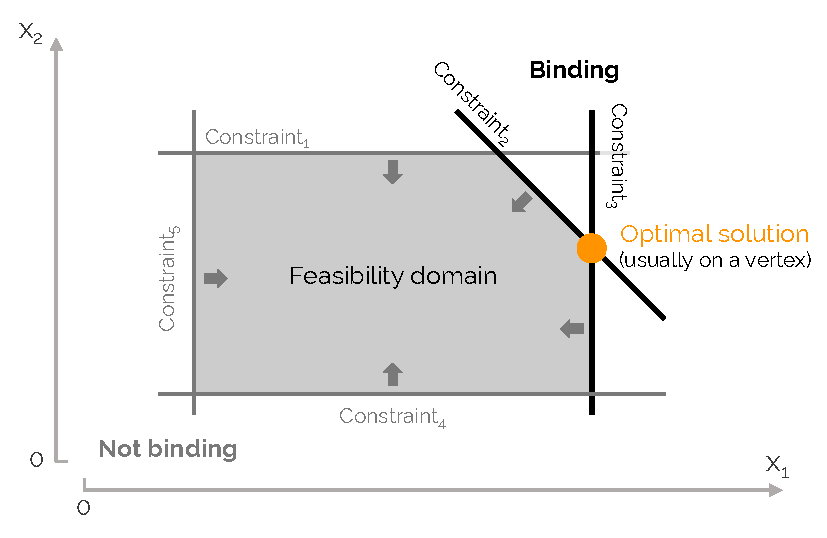
\includegraphics[width=0.7\textwidth]{Binding_constr.pdf}
\caption{Binding versus non-binding constraints. In LP where the feasibility domain is non-empty and bounded, the constraints defined a convex feasibility domain in the space of variables (here, x$_1$ and x$_2$). The optimal solution usually locates on a vertex of this domain, \ie the intersection of several constraints (here, constraints 2 and 3) limiting the solution. These constraints are considered as binding, \ie having a limiting impact on the optimal solution.}
\label{fig:Binding_constr}
\end{figure}

\section{Chapter 5 - Principal Component Analysis}
\label{PCA}

\begin{mdframed}[style=comment] % Comment from the reviewer
{\color{orange} \textbf{Stefano}} - p. 101: you mention different definitions of “robustness”: which one do you use in your work?
\end{mdframed}

\noindent 

\begin{mdframed}[style=manuscript] % Modification brought to the manuscript

\end{mdframed}

\begin{mdframed}[style=comment] % Comment from the reviewer
{\color{orange} \textbf{Stefano}} - p. 109: how is Gamma-robustness implemented here? It seems like it is in some sense “manually” forced? Explain better how the ROB solution is derived.
\end{mdframed}

\noindent 

\begin{mdframed}[style=manuscript] % Modification brought to the manuscript

\end{mdframed}


\subsection{Confusion with the word PC}
\label{Confusion_PC_wording}


\begin{mdframed}[style=comment] % Comment from the reviewer
{\color{violet} \textbf{Christophe}} When using the word ``component'', there seems to be a confusion and it is not always easy to understand if you refer to the vector or the coefficient related to one of the original variable.
\end{mdframed}

\noindent The confusion probably comes from the fact a Principal Component (PC) actually represents an eigenvector of the covariance matrix. This vector is, by definition, composed of \textbf{components}, each of them being a coefficient related to a specific original variable. Parts where the word ``component'' is not directly linked to ``vector'', ``eigenvector'' or ``PC'' are those that could mislead the reader. Modifications have been brought to these parts.

{\color{blue} End of second paragraph of section 1.4.1}:

\begin{mdframed}[style=manuscript] % Modification brought to the manuscript
Moreover, this means that \textbf{the coefficient} $\alpha_{ki}$, \ie the component of $\bm{\alpha}_{\mathbf{k}}$ related to the $i^{\text{th}}$ original variable, $x_i$,  gives its weight in the $k^{\text{th}}$ PC, \ie $z_k$. 
\end{mdframed}

\section{Conclusion}
\label{Conclusion}

\begin{mdframed}[style=comment] % Comment from the reviewer
{\color{orange} \textbf{Stefano}} \& {\color{purple} \textbf{Sylvain}} - p. 119: the statement mentioning the ``major added value of the perfect foresight'' approach seems surprising and needs to be clarified. 
\end{mdframed}

\noindent 

\begin{mdframed}[style=manuscript] % Modification brought to the manuscript

\end{mdframed}

\begin{mdframed}[style=comment] % Comment from the reviewer
{\color{teal} \textbf{Stefan}} - The conclusion is a summary and should rather be a discussion (\eg discard coal as soon as possible is obvious).
\end{mdframed}

\noindent To explain in the definition of the action {\color{blue} }. 

\begin{mdframed}[style=manuscript] % Modification brought to the manuscript 

\end{mdframed}


\clearpage
\def\bibfont{\scriptsize}
\bibliography{../bib_thesis.bib}
\normalsize

\end{document}